
% \begin{frame}{\href{section4/animation/hyperelasticity_velo/video.mp4}{Plane strain hyperelasticity -- Neo-Hookean material}}
%   \footnotesize Comparison with FEM \cite{Abaqus}--MPM--DGMPM
%   \begin{overprint}
%     \onslide<1>
%     \vspace{0.5cm}
%     \begin{center}
%       \input{section4/pgfFigures/2d_squareHE}
%       \footnotesize $v^d = -1000 \: m/s$
%     \end{center}

%     \onslide<2>
%     \vspace{0.cm}
%     \begin{center}
%       % \movie[width=1.\linewidth,showcontrols,loop]{\input{section4/pgfFigures/2d_square}}{section4/animation/hyperelasticity_velo/video.mp4}
%       \movie[height = 0.6\paperheight,width=0.9\linewidth, showcontrols,loop,poster,autostart]{%\input{section4/pgfFigures/2d_squareHE}
%       }{section4/animation/hyperelasticity_velo/video.mp4}
%     \end{center}
%   \end{overprint}
%   \footnoteCite{Abaqus}
% \end{frame}

\begin{frame}
  \footnotesize Comparison with FEM--MPM--DGMPM (variational constitutive update \cite{LaurentVariational})
  \begin{overprint}
    \onslide<1>
    \begin{columns}
      \begin{column}{0.49\textwidth}
        \vspace{0.18cm}
        \centering
          \begin{tikzpicture}[scale=0.9]
  \draw[thick] (0,0) --(3,0)--(3,3)--(0,3)--(0,0);
  \foreach \x in {0.5,1.,...,2.5} 
  \draw(\x,-0.2)circle(0.2);
  \foreach \x in {0.25,0.75,...,2.75} 
  \draw(-0.2,\x)circle(0.2);
  \draw(0,-0.4)--(3.,-0.4);
  \draw(-.4,0)--(-.4,3);
  \fill [pattern=north east lines](0.0,-0.8)rectangle+(3,0.4);
  \fill [pattern=north east lines](-.8,0.)rectangle+(0.4,3);
  \draw[>=stealth,<->](0,3.1)--node[above=1pt]{\footnotesize $l=3 \: m$}(3,3.1);
  %\draw[>=stealth,<->](0.1,0)--node[right=1pt]{\footnotesize $a=1 \: m$}(0.1,1);
  % \foreach \x in {0.,0.25,...,1} 
  % \draw[>=stealth,<-] (-0.5,\x)--(0.,\x);
  % \node(a)at(-1.75,0.5){\footnotesize $\vect{v}=\matrice{v^d\\0 \\0}$}; 
  \node[right] (a) at(3.25,1.5){\footnotesize $\vect{v}(\vect{x},t=0)=\matrice{v^d\\0 \\0}$}; 
  \draw[>=stealth,->](-2.5,2)--(-1.5,2)node(a)[anchor=north]{\footnotesize $\vect{e}_1$};
  \draw[>=stealth,->](-2.5,2)--(-2.5,3)node(a)[anchor=south]{\footnotesize $\vect{e}_2$};
\end{tikzpicture}


%%% Local Variables:
%%% mode: latex
%%% TeX-master: "../../presentation"
%%% End:

          \footnotesize $v^d = -300 \: \text{m/s}$
        \end{column}
      \begin{column}{0.49\textwidth}
        
      \end{column}
    \end{columns}
    \vspace{0.22cm}
    \footnoteCite{LaurentVariational}
    \onslide<2>
    \begin{columns}
      \begin{column}{0.49\textwidth}
        \centering
        \begin{tikzpicture}[scale=0.9]
  \draw[thick] (0,0) --(3,0)--(3,3)--(0,3)--(0,0);
  \foreach \x in {0.5,1.,...,2.5} 
  \draw(\x,-0.2)circle(0.2);
  \foreach \x in {0.25,0.75,...,2.75} 
  \draw(-0.2,\x)circle(0.2);
  \draw(0,-0.4)--(3.,-0.4);
  \draw(-.4,0)--(-.4,3);
  \fill [pattern=north east lines](0.0,-0.8)rectangle+(3,0.4);
  \fill [pattern=north east lines](-.8,0.)rectangle+(0.4,3);
  \draw[>=stealth,<->](0,3.1)--node[above=1pt]{\footnotesize $l=3 \: m$}(3,3.1);
  %\draw[>=stealth,<->](0.1,0)--node[right=1pt]{\footnotesize $a=1 \: m$}(0.1,1);
  % \foreach \x in {0.,0.25,...,1} 
  % \draw[>=stealth,<-] (-0.5,\x)--(0.,\x);
  % \node(a)at(-1.75,0.5){\footnotesize $\vect{v}=\matrice{v^d\\0 \\0}$}; 
  \node[right] (a) at(3.25,1.5){\footnotesize $\vect{v}(\vect{x},t=0)=\matrice{v^d\\0 \\0}$}; 
  \draw[>=stealth,->](-2.5,2)--(-1.5,2)node(a)[anchor=north]{\footnotesize $\vect{e}_1$};
  \draw[>=stealth,->](-2.5,2)--(-2.5,3)node(a)[anchor=south]{\footnotesize $\vect{e}_2$};
\end{tikzpicture}


%%% Local Variables:
%%% mode: latex
%%% TeX-master: "../../presentation"
%%% End:

          \footnotesize $v^d = -300 \: \text{m/s}$
      \end{column}
      \begin{column}{0.49\textwidth}
        \centering
        % 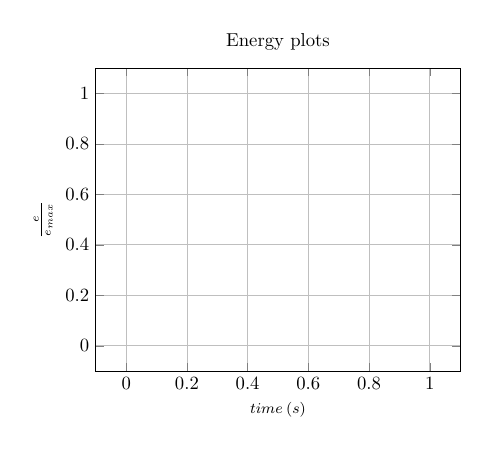
\begin{tikzpicture}[scale=.675]
\begin{axis}[xlabel=\footnotesize $\text{time} \: (s)$,ylabel=\footnotesize $\frac{e}{e_{max}}$,ymajorgrids=true,xmajorgrids=true,legend pos=outer north east,title={Energy plots}]
%\addplot[Red,very thick,mark=none,dashed,mark size=2pt] table[x=Time,y=q1(Y)] {section4/csvFiles/topNode_dgmpm0.0.csv};
%\addplot[Orange,very thick,mark=none,mark size=2pt] table[x=Time,y=q1(Y)] {section4/csvFiles/topNode0.0.csv};
%\addplot[Orange,very thick,mark=none,densely dotted,mark size=3pt] ;
%\legend{mpm-flip 1ppc -- CFL=0.5,mpm-flip 2ppc -- CFL=0.5,mpm-pic 2ppc }
\end{axis}
\end{tikzpicture}
%%% Local Variables:
%%% mode: latex
%%% TeX-master: "../../presentation"
%%% End:

        \begin{tikzpicture}[scale=.85]
\begin{axis}[xlabel=\footnotesize $x \: (m)$,ylabel=\footnotesize $\Pi_{11}$ (Pa),ymajorgrids=true,xmajorgrids=true,legend pos=north west,title={Stress}]% $t=6\times 10^{-4}$s
\addplot[Blue,very thick,mark=x,mark size=2pt,only marks] table[x=Points:0,y=Piola_11] {section4/csvFiles/bottom_dgmpm.csv};
\addplot[Orange,very thick,mark=none,mark size=2pt] table[x=Points:0,y=Piola_Stress:0] {section4/csvFiles/bottom_fem.csv};
\addplot[Red,very thick,mark=square,mark size=2pt,only marks] table[x=Points:0,y=mpm_S11] {section4/csvFiles/bottom_mpm.csv};
\legend{dgmpm--CFL=0.9,fem--CFL=0.9,mpm--CFL=0.7}
\end{axis}
\end{tikzpicture}
%%% Local Variables:
%%% mode: latex
%%% TeX-master: "../../presentation"
%%% End:

      \end{column}
    \end{columns}
    \footnoteCite{LaurentVariational}
  \end{overprint}
\end{frame}

\begin{frame}{\href{section4/animation/hyperelastoplasticity/epeq.mp4}{Plane strain hyperelastoplasticity -- Hencky material; linear isotropic hardening}}
  \begin{center}
    \movie[height = 0.7\paperheight,width=1.\linewidth, showcontrols,poster,loop,autostart]{%\begin{tikzpicture}[scale=0.9]
  \draw[thick] (0,0) --(3,0)--(3,3)--(0,3)--(0,0);
  \foreach \x in {0.5,1.,...,2.5} 
  \draw(\x,-0.2)circle(0.2);
  \foreach \x in {0.25,0.75,...,2.75} 
  \draw(-0.2,\x)circle(0.2);
  \draw(0,-0.4)--(3.,-0.4);
  \draw(-.4,0)--(-.4,3);
  \fill [pattern=north east lines](0.0,-0.8)rectangle+(3,0.4);
  \fill [pattern=north east lines](-.8,0.)rectangle+(0.4,3);
  \draw[>=stealth,<->](0,3.1)--node[above=1pt]{\footnotesize $l=3 \: m$}(3,3.1);
  %\draw[>=stealth,<->](0.1,0)--node[right=1pt]{\footnotesize $a=1 \: m$}(0.1,1);
  % \foreach \x in {0.,0.25,...,1} 
  % \draw[>=stealth,<-] (-0.5,\x)--(0.,\x);
  % \node(a)at(-1.75,0.5){\footnotesize $\vect{v}=\matrice{v^d\\0 \\0}$}; 
  \node[right] (a) at(3.25,1.5){\footnotesize $\vect{v}(\vect{x},t=0)=\matrice{v^d\\0 \\0}$}; 
  \draw[>=stealth,->](-2.5,2)--(-1.5,2)node(a)[anchor=north]{\footnotesize $\vect{e}_1$};
  \draw[>=stealth,->](-2.5,2)--(-2.5,3)node(a)[anchor=south]{\footnotesize $\vect{e}_2$};
\end{tikzpicture}


%%% Local Variables:
%%% mode: latex
%%% TeX-master: "../../presentation"
%%% End:

    }{section4/animation/hyperelastoplasticity/epeq.mp4}
  \end{center}
\end{frame}

\begin{frame}{\href{section4/animation/hyperelastoplasticity/stress.mp4}{Plane strain hyperelastoplasticity -- Hencky material; linear isotropic hardening}}
  \begin{center}
    \movie[height = 0.7\paperheight,width=1.\linewidth, showcontrols,poster,loop,autostart]{%\begin{tikzpicture}[scale=0.9]
  \draw[thick] (0,0) --(3,0)--(3,3)--(0,3)--(0,0);
  \foreach \x in {0.5,1.,...,2.5} 
  \draw(\x,-0.2)circle(0.2);
  \foreach \x in {0.25,0.75,...,2.75} 
  \draw(-0.2,\x)circle(0.2);
  \draw(0,-0.4)--(3.,-0.4);
  \draw(-.4,0)--(-.4,3);
  \fill [pattern=north east lines](0.0,-0.8)rectangle+(3,0.4);
  \fill [pattern=north east lines](-.8,0.)rectangle+(0.4,3);
  \draw[>=stealth,<->](0,3.1)--node[above=1pt]{\footnotesize $l=3 \: m$}(3,3.1);
  %\draw[>=stealth,<->](0.1,0)--node[right=1pt]{\footnotesize $a=1 \: m$}(0.1,1);
  % \foreach \x in {0.,0.25,...,1} 
  % \draw[>=stealth,<-] (-0.5,\x)--(0.,\x);
  % \node(a)at(-1.75,0.5){\footnotesize $\vect{v}=\matrice{v^d\\0 \\0}$}; 
  \node[right] (a) at(3.25,1.5){\footnotesize $\vect{v}(\vect{x},t=0)=\matrice{v^d\\0 \\0}$}; 
  \draw[>=stealth,->](-2.5,2)--(-1.5,2)node(a)[anchor=north]{\footnotesize $\vect{e}_1$};
  \draw[>=stealth,->](-2.5,2)--(-2.5,3)node(a)[anchor=south]{\footnotesize $\vect{e}_2$};
\end{tikzpicture}


%%% Local Variables:
%%% mode: latex
%%% TeX-master: "../../presentation"
%%% End:

    }{section4/animation/hyperelastoplasticity/stress.mp4}
  \end{center}
\end{frame}

%%% Local Variables:
%%% mode: latex
%%% TeX-master: "../presentation"
%%% End:
